\documentclass[aspectratio=169]{beamer}
\usepackage{ctex}
\usepackage{graphicx}
\usepackage{tikz}
\usepackage{booktabs}

% 主题设置
\usetheme{Madrid}
\usecolortheme{default}

% 标题信息
\title{轨道向前,车轮转型}
\subtitle{我与我的新时代——聚焦公交与地铁变迁}
\author{陈恪瑾}
\date{2025年11月21日}
\institute{武汉交通的时代故事}

\begin{document}

% ==================== 封面页 ====================
\begin{frame}[plain]
    \titlepage
    \begin{center}
        \begin{columns}
            \column{0.5\textwidth}
            \centering
            \includegraphics[width=0.9\textwidth]{pictures/Page1/old_bus.png}
            
            \column{0.5\textwidth}
            \centering
            \includegraphics[width=0.9\textwidth]{pictures/Page1/new_subway.png}
        \end{columns}
    \end{center}
\end{frame}

% ==================== 目录页 ====================
\begin{frame}{目录}
    \tableofcontents
\end{frame}

% ==================== 第一部分 ====================
\section{记忆开篇:武汉公交的传说}

\begin{frame}{记忆开篇:武汉公交的传说}
    \begin{center}
        \Large 在过去的武汉街头,流传着这样一种传说。
    \end{center}
    
    \vspace{1em}
    
    \begin{block}{}
        \centering
        \large "天上战斗机,地上521。"
    \end{block}
    
    \begin{block}{}
        \centering
        \large "集齐四辆521在洪山广场上转圈,可以打开时空之门。"
    \end{block}
    
    \begin{block}{}
        \centering
        \large "武汉521,公路上的F1。"
    \end{block}
    
    \vspace{1em}
    
    \begin{center}
        说的不是什么暗号,而是"飙车时车轮起过火"的武汉521路公交车。
        
        \vspace{1em}
        % 视频占位符
        \fbox{\parbox{0.7\textwidth}{\centering [视频:521.mp4]}}
    \end{center}
\end{frame}

% ==================== 第二部分 ====================
\section{核心对比:公交"退"与地铁"兴"}

% Page 4: 数据对比
\begin{frame}{公交"退"与地铁"兴"}
    \begin{columns}
        \column{0.75\textwidth}
        % 折线图
        \begin{center}
            \begin{tikzpicture}[scale=1.0]
                % 坐标轴
                \draw[->] (0,0) -- (7,0) node[right] {年份};
                \draw[->] (0,0) -- (0,5) node[above] {占比(\%)};
                
                % 刻度
                \foreach \x/\year in {0/2011, 1.5/2013, 3/2015, 4.5/2017, 6/2019}
                    \draw (\x,0.1) -- (\x,-0.1) node[below] {\tiny \year};
                \foreach \y/\val in {1/20, 2/40, 3/60, 4/80}
                    \draw (0.1,\y) -- (-0.1,\y) node[left] {\small \val};
                
                % 公交线(下降)
                \draw[thick,blue,->] (0,3.7) -- (6,2.4);
                \node[blue] at (0.8,4.0) {\small 公交};
                \node[blue] at (0.8,3.6) {\small 74.7\%};
                \node[blue] at (5.2,2.1) {\small 47.7\%};
                
                % 地铁线(上升)
                \draw[thick,red,->] (0,0.2) -- (6,2.05);
                \node[red] at (0.8,0) {\small 地铁};
                \node[red] at (0.8,-0.4) {\small 3.9\%};
                \node[red] at (5.2,2.4) {\small 41\%};
            \end{tikzpicture}
        \end{center}
        
        \column{0.25\textwidth}
        \large 常规公交客运占公共交通客运总量的比重由2011年\textbf{74.7\%}下降到2019年\textbf{47.7\%},
        
        \vspace{0.5em}
        
        同期轨道交通占比由\textbf{3.9\%}提升至\textbf{41\%}
        
        \vspace{1em}
    \end{columns}
\end{frame}

% Page 5: 公交"退"
\begin{frame}{公交"退"}
    \begin{center}
        \LARGE \textbf{公交停运,优化重复线路}
        
        \vspace{1em}
        
        \begin{columns}
            \column{0.33\textwidth}
            \centering
            \includegraphics[width=\textwidth]{pictures/Page5/1.png}
            
            \column{0.33\textwidth}
            \centering
            \includegraphics[width=\textwidth]{pictures/Page5/2.png}
            
            \column{0.33\textwidth}
            \centering
            \includegraphics[width=\textwidth]{pictures/Page5/3.png}
        \end{columns}
        
        \vspace{1em}
        
        \includegraphics[width=0.7\textwidth]{pictures/Page5/4.png}
    \end{center}
\end{frame}

% Page 6: 大站快线
\begin{frame}{公交"退":转型升级}
    \begin{center}
        \LARGE \textbf{开设大站快线"K字头"}
        
        \vspace{1em}
        
        \includegraphics[width=0.7\textwidth]{pictures/Page6/1.png}
    \end{center}
\end{frame}

% Page 7: 定制公交
\begin{frame}{公交"退":精准服务}
    \begin{center}
        \LARGE \textbf{开设定制公交,满足特定群体需求}
        
        \vspace{1em}
        
        \includegraphics[width=0.7\textwidth]{pictures/Page7/1.png}
    \end{center}
\end{frame}

% Page 8: 地铁"兴"
\begin{frame}[allowframebreaks]{地铁"兴"}
    \begin{block}{规模成就}
        运营里程达 \textbf{518 公里}(含鄂州延伸段),跻身\textbf{世界前十},覆盖武汉全域 + 鄂州葛店,无缝衔接机场、三大火车站,跨江跨区客流占比超 40\%。
    \end{block}
    
    \begin{block}{跨江技术}
        2 号线开创\textbf{全国地铁穿长江先例},后续累计 6 穿长江,2 穿汉江,最深盾构深度达地下 30 米
    \end{block}
    
    \begin{block}{自动驾驶}
        2021 年开通的 5 号线为武汉首条真正无驾驶室的\textbf{全自动驾驶线路},实现列车唤醒、运营、回库全流程自动化,故障率降至百万列公里 0.7 次,准点率达 99.99\%,较普通线路效率提升 7.3\%。
    \end{block}
    
    \framebreak
    
    \begin{block}{便民服务}
        2024 年夏季延长 2、5 号线运营至凌晨,跨年夜连续运营 21 小时,运送夜间乘客 24.18 万人次,司门口黄鹤楼站年客流超千万,成为 "地铁 + 文旅" 标杆。
    \end{block}
    
    \begin{block}{工程创新}
        2 号线十汉区间攻克 136 个溶洞(最大直径 13.8 米)的岩溶发育区,创新 "先填后掘 + 镶齿滚刀" 技术,为同类工程提供范本。
    \end{block}

    \begin{block}{绿色低碳}     
        采用再生制动能量回收系统,年节电超 1.2 亿千瓦时,车站应用光伏供电、节能照明等绿色技术,碳减排量等效每年少烧 5 万吨标准煤,获评 “国家级绿色交通示范工程”。
    \end{block}
\end{frame}

% Page 9: 地铁网络扩展
\begin{frame}{地铁"兴":网络扩展}
    \begin{center}
        \LARGE \textbf{地铁线路快速扩展,覆盖主要城区}
        
        \vspace{1em}
        
        \includegraphics[width=0.6\textwidth]{pictures/Page9/1.png}
    \end{center}
\end{frame}

% ==================== 第三部分 ====================
\section{时代逻辑:变迁背后的密码}

% Page 10: 时代逻辑
\begin{frame}{时代逻辑:变迁背后的密码}
    \begin{block}{城市发展需求}
        武汉从 "\textbf{三镇分立}" 到 "\textbf{都市圈融合}"(建成区翻倍),市民需 "快、稳、舒适" 出行:地铁 37 分钟平均通勤时耗(800 米覆盖率全国第三),公交 "拥堵迟到" 痛点凸显。
    \end{block}
    
    \begin{block}{绿色发展导向}
        绿色政策(如 "武碳江湖")更青睐地铁。
    \end{block}
    
    \begin{block}{互补共生}
        两者形成 "\textbf{地铁骨干 + 公交接驳}" 互补网,本质是新时代交通向 "\textbf{高效、精准、绿色}" 升级的缩影。
    \end{block}
\end{frame}

% ==================== 第四部分 ====================
\section{我的共鸣:成长与交通同频}

% Page 11: 我的共鸣
\begin{frame}{我的共鸣:成长与交通同频}
    \begin{block}{536路的变迁}
        536路从汉口火车站到光谷大道,后改线为光谷广场到武汉未来科技城,到如今停运
    \end{block}
    
    \begin{block}{地铁2号线的陪伴}
        地铁2号线东沿线经过华中科技大学与家门口
    \end{block}
    
    \begin{block}{雄楚大道BRT改造}
        雄楚大道BRT改造使得738配车从双层车到10m单层车到如今6m小巴
    \end{block}
    
    \vspace{1em}
    \begin{center}
        \large 这些变化,见证了我的成长,也映射着城市交通的迭代升级
    \end{center}
\end{frame}

% ==================== 第五部分 ====================
\section{总结:交通里的新时代}

% Page 12: 总结
\begin{frame}[allowframebreaks]{总结:交通里的新时代}
    \begin{block}{核心观点}
        \large 公交 “退” 是迭代,地铁 “兴” 是需求,二者互补共生
    \end{block}
    
    公交"退"与地铁"兴",是城市交通的\textbf{迭代共生},更是国家转型的生动注脚——这背后,藏着新时代的发展智慧与青年担当。
    
    \vspace{0.5em}
    
    公交的"退",是\textbf{主动迭代而非退场}:以大站快车、定制公交精准对接需求,用地铁接驳线填补服务空白,既疏解拥堵,又守好民生温度。

    \vspace{1em}
    
    地铁的"兴",是\textbf{顺势而为更是担当}:以大运量、高速度承载城市活力,成为发展的动力引擎。一"退"一"兴",是"\textbf{以人民为中心}"的鲜活实践。
    
    \vspace{0.5em}
    
    这恰是我们与时代的相处之道:青年如地铁,可凭专业硬核攻坚;如定制公交,可精准补位暖心。不必强求一律的"高速",但需练就精准作为的本领,在时代大局中实现价值。
    
    \framebreak
    
    \begin{columns}
        \column{0.5\textwidth}
        \centering
        \includegraphics[width=\textwidth]{pictures/Page12/1.png}
        
        \column{0.5\textwidth}
        新时代是\textbf{各扬所长的交响},\\
        青年与时代是\textbf{双向成就的征程}。
        
        \vspace{1em}
        
        读懂交通的互补之道,便明晰使命:\\
        以地铁之锐突破,以公交之智应变,\\
        与时代同频共振。
        
        \vspace{1em}
        
        \Large \textbf{让我们与时代并肩,\\
        迭代中守初心,共生中勇担当,\\
        共赴美好新征程!}
    \end{columns}
\end{frame}

% ==================== 致谢页 ====================
\begin{frame}[plain]
    \begin{center}
        \Huge \textbf{感谢聆听!}
        
        \vspace{1em}
        \includegraphics[width=0.8\textwidth]{pictures/Page13/1.png}
        
        \vspace{1em}
        \large 以交通为笔,写我们的新时代故事
    \end{center}
\end{frame}

\end{document}